\section{Process ID Example}
\label{sec:pid}
The illustration of asymmetric fault implementation can be seen through a simple example where 4 nodes report to each other their own process ID (PID). Each node has a 1-3 connection and thus each node is a candidate for an asymmetric fault. Given this architecture, a top level contract of the system is simply that all nodes report and see the correct PID of all other nodes. Naturally in the absence of faults, this holds. But when one asymmetric fault is introduced on any of the nodes, this contract cannot be verified. What is desired is a protocol in which all nodes agree on a value (correct or arbitrary) for all PIDs. 

\subsection{The Agreement Protocol Behavioral Implementation}
In order to mitigate this problem, special attention must be given to the behavioral model. Using the strategies outlined in previous research~\cite{bracha1987asynchronous,Driscoll-Byzantine-Fault}, the agreement protocol is specified in AGREE to create a model resilient to one active Byzantine fault. 

The objective of the agreement protocol is for all correct (non-failed) nodes to eventually reach agreement on the PID values of the other nodes. There are $n$ nodes, possibly $f$ failed nodes. The protocol requires $n > 3f$ nodes to handle a single fault. The point is to achieve distributed agreement and coordinated decisions.
The properties that must be verified in order to prove the protocol works as desired are as follows: 
\begin{itemize}
	\item All correct (non-failed) nodes eventually reach a decision regarding the value they have been given.  In this solution, nodes will agree in $f+1$ time steps or rounds of communication.   
	\item If the source node is correct, all other correct nodes agree on the value that was originally sent by the source.  
	\item If the source node is failed, all other nodes must agree on some predetermined default value.  
\end{itemize}

The updated architecture of the PID example is shown in Figure~\ref{fig:PIDArch}. 
\begin{figure}[!htb]
        \center{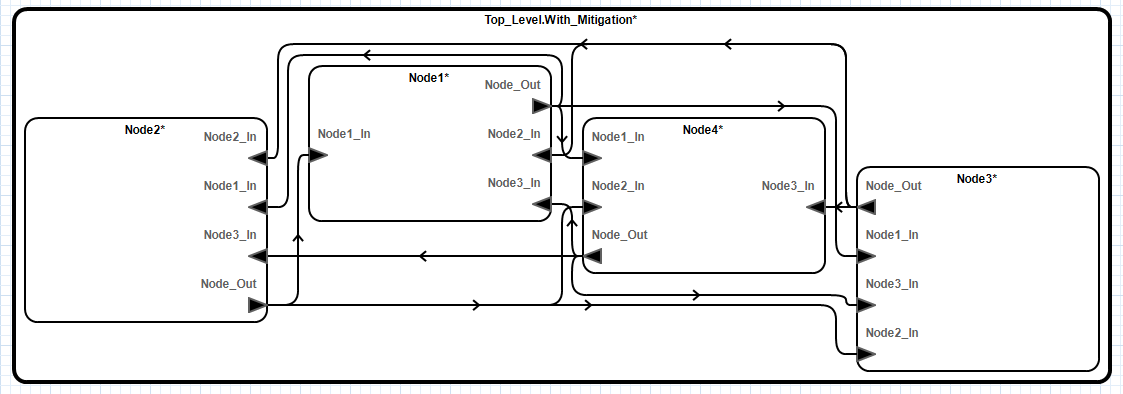
\includegraphics[width=\textwidth] {images/PIDArch.png}}
        \caption{\label{fig:PIDArch} Updated PID Example Architecture}
\end{figure}

Each node reports its own PID to all other nodes in the first round of communication. In the second round, each node informs the others what they saw in terms of %everyones
everyone's PIDs. %Thus, new connections are added for this second round of communication.
The outputs from a node are described in Figure~\ref{fig:NodeOutputsPID}. %\janet{The figure needs to be updated, as node 2 sends to node 1, 2, 3; and node 3 sends to node 1, 2, 4; and node 4 sends to node 1, 2, 3}
\begin{figure}[!htb]
        \center{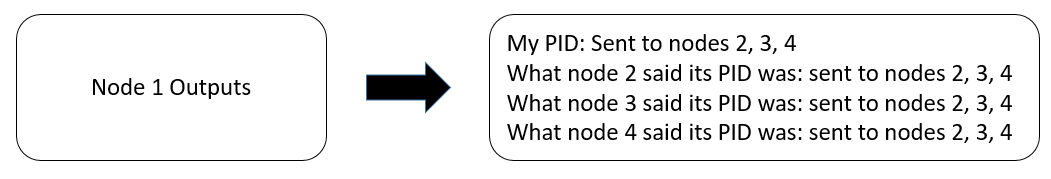
\includegraphics[width=0.9\textwidth] {images/NodeOutputsPID.png}}
        \caption{\label{fig:NodeOutputsPID} Description of the Outputs of Each Node in the PID Example}
\end{figure}
%These new connections 
These outputs are modeled as a nested data implementation in AADL and each field corresponds to a PID from a node. The AADL code fragment defining this data implementation is shown in Figure~\ref{fig:PIDNodeData}.

\begin{figure}[!htb]
        \center{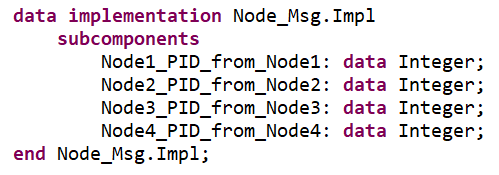
\includegraphics[width=0.7\textwidth] {images/PIDNodeData.png}}
        \caption{\label{fig:PIDNodeData} Data Implementation in AADL for Node Outputs}
\end{figure}

The fault definition for %that is inserted explicitly into the model is connected to 
each node's output and can effect the data fields arbitrarily. This is a nondeterministic fault in two ways. It is nondeterministic how many receiving nodes see incorrect values and it is nondeterministic how many of the data fields are affected by this fault. This can be accomplished through the fault definition shown in Figure~\ref{fig:PIDFaultNode} and the fault node definition in Figure~\ref{fig:PIDFaultDef}. 

\begin{figure}[!htb]
        \center{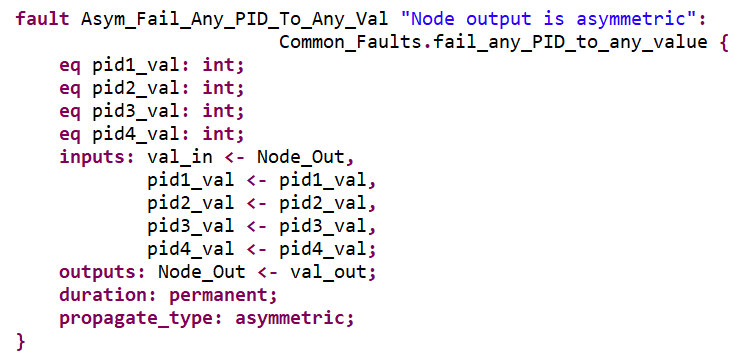
\includegraphics[width=0.9\textwidth] {images/PIDFaultNode.png}}
        \caption{\label{fig:PIDFaultNode} Fault Definition on Node Outputs for PID Example}
\end{figure}

\begin{figure}[!htb]
        \center{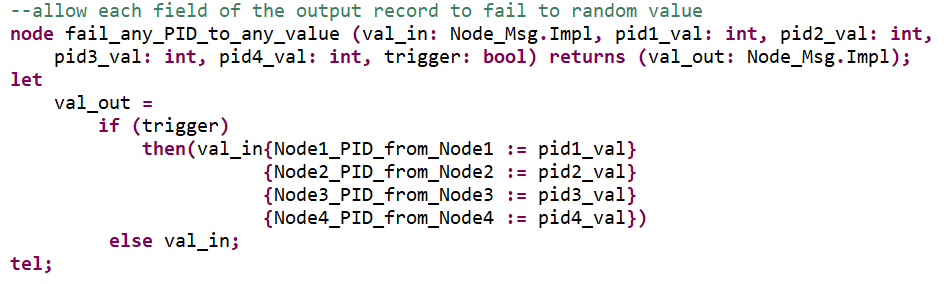
\includegraphics[width=0.9\textwidth] {images/PIDFaultDef.png}}
        \caption{\label{fig:PIDFaultDef} Fault Node Definition for PID Example}
\end{figure}

Once the fault model is in place, the implementation in AGREE of the agreement protocol is developed. As stated previously, there are two cases that must be considered in the contracts of this system. 
\begin{itemize}
	\item In the case of no active faults, all nodes must agree on the correct PID of all other nodes. 
	\item In the case of an active fault on a node, all non-failed nodes must agree on a PID for all other nodes. 
\end{itemize}

These requirements are encoded in AGREE through the use of the following contracts. Figure~\ref{fig:PIDContract1} and Figure~\ref{fig:PIDContract2} show example contracts regarding Node 1 PID. There are similar contracts for each node's PID. 
\begin{figure}[!htb]
        \center{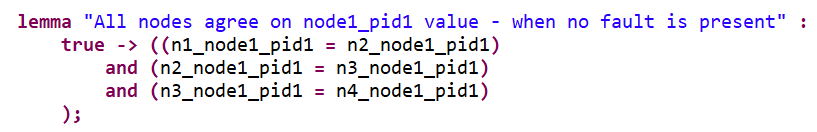
\includegraphics[width=0.9\textwidth] {images/PIDContract1.png}}
        \caption{\label{fig:PIDContract1} Agreement Protocol Contract in AGREE for No Active Faults}
\end{figure}

\begin{figure}[!htb]
        \center{\includegraphics[width=0.9\textwidth] {images/PIDCOntract2.png}}
        \caption{\label{fig:PIDContract2} Agreement Protocol Contract in AGREE Regarding Non-failed Nodes}
\end{figure}


\textbf{Referencing Fault Activation Status}
To fully implement the agreement protocol, it must be possible to describe whether or not a component has failed; this is performed through the use of a \textit{fault activation statement}. The user first defines \textit{eq} variables in AGREE that will correspond to specific faults in components. Each of the \textit{eq} variables declared in AGREE (i.e., \textit{n1\_failed, n2\_failed, n3\_failed, n4\_failed}) is linked to the fault activation status of the \textit{Asym\_Fail\_Any\_PID\_To\_Any\_Value} fault defined in a node subcomponent instance of the %top level 
AADL system implementation (i.e., \textit{node1}, \textit{node2}, \textit{node3}, \textit{node4}). The fault activation statements for the PID example are shown in Figure~\ref{fig:PID_faultActivationStmt}.

\begin{figure}[!htb]
        \center{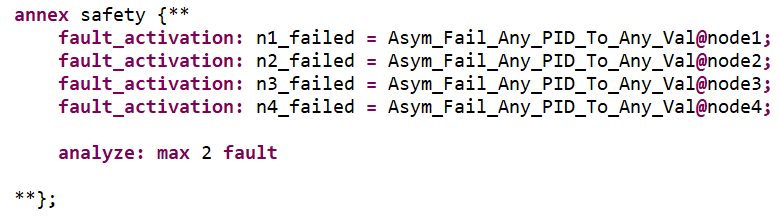
\includegraphics[width=0.9\textwidth] {images/PID_faultActivationStmt.png}}
        \caption{\label{fig:PID_faultActivationStmt} Fault Activation Statement in PID Example}
\end{figure}

\subsection{Nominal and Fault Model Analysis}
The nominal model verification shows that all properties are valid. Upon running verification in the presence of faults with maximum one active fault, the first four properties stating that all nodes agree on the correct value (Figure~\ref{fig:PIDContract1}) fail. This is expected since this property is specific to the case when no faults are present in the model. The remaining 4 top level properties (Figure~\ref{fig:PIDContract2}) state that all non-failed nodes reach agreement in two rounds of communication. These are verified valid when any one asymmetric fault is present. This shows that the agreement protocol was successful in eliminating a single point of asymmetric failure from the model. Furthermore, when changing the number of allowed faults to two, these properties do not hold. This is expected given the theoretical result that $3f+1$ nodes are required in order to be resilient to $f$ faults and that $f+1$ rounds of communication are needed for successful protocol implementation.

A summary of the results follows. 
\begin{itemize}
	\item Nominal model: All top level guarantees are verified. All nodes output the correct value and all agree. 
	\item Fault model with one active fault: The first four guarantees fail (when no fault is present, all nodes agree: shown in Figure~\ref{fig:PIDContract1}). This is expected if faults are present. The last four guarantees (all non-failed nodes agree) are verified as true with one active fault. 
	\item Fault model with two active faults: All 8 guarantees fail. This is expected since in order to be resilient up to two active faults ($f=2$), we would need $3f + 1 = 7$ nodes and $f+1 = 3$ rounds of communication. 
\end{itemize}

This example illustrates the correct handling of such faults and how to utilize the capabilities of the safety annex to model asymmetric failures and test that a system is resilient to such faults. 
